\documentclass[../bericht.tex]{subfiles}

\begin{document}

  \begin{appendices}

    \section{Netzteil-Kennlinie}
    \label{sec:netzteil-kennlinie}
      \Cref{fig:netzteil-kennlinie} zeigt die für die Berechnung der Laserschwelle in \cref{subsec:laserschwelle} verwendete Charakterisitk des verwendeten Netzteils.

      \begin{figure}[H]
        \centering
        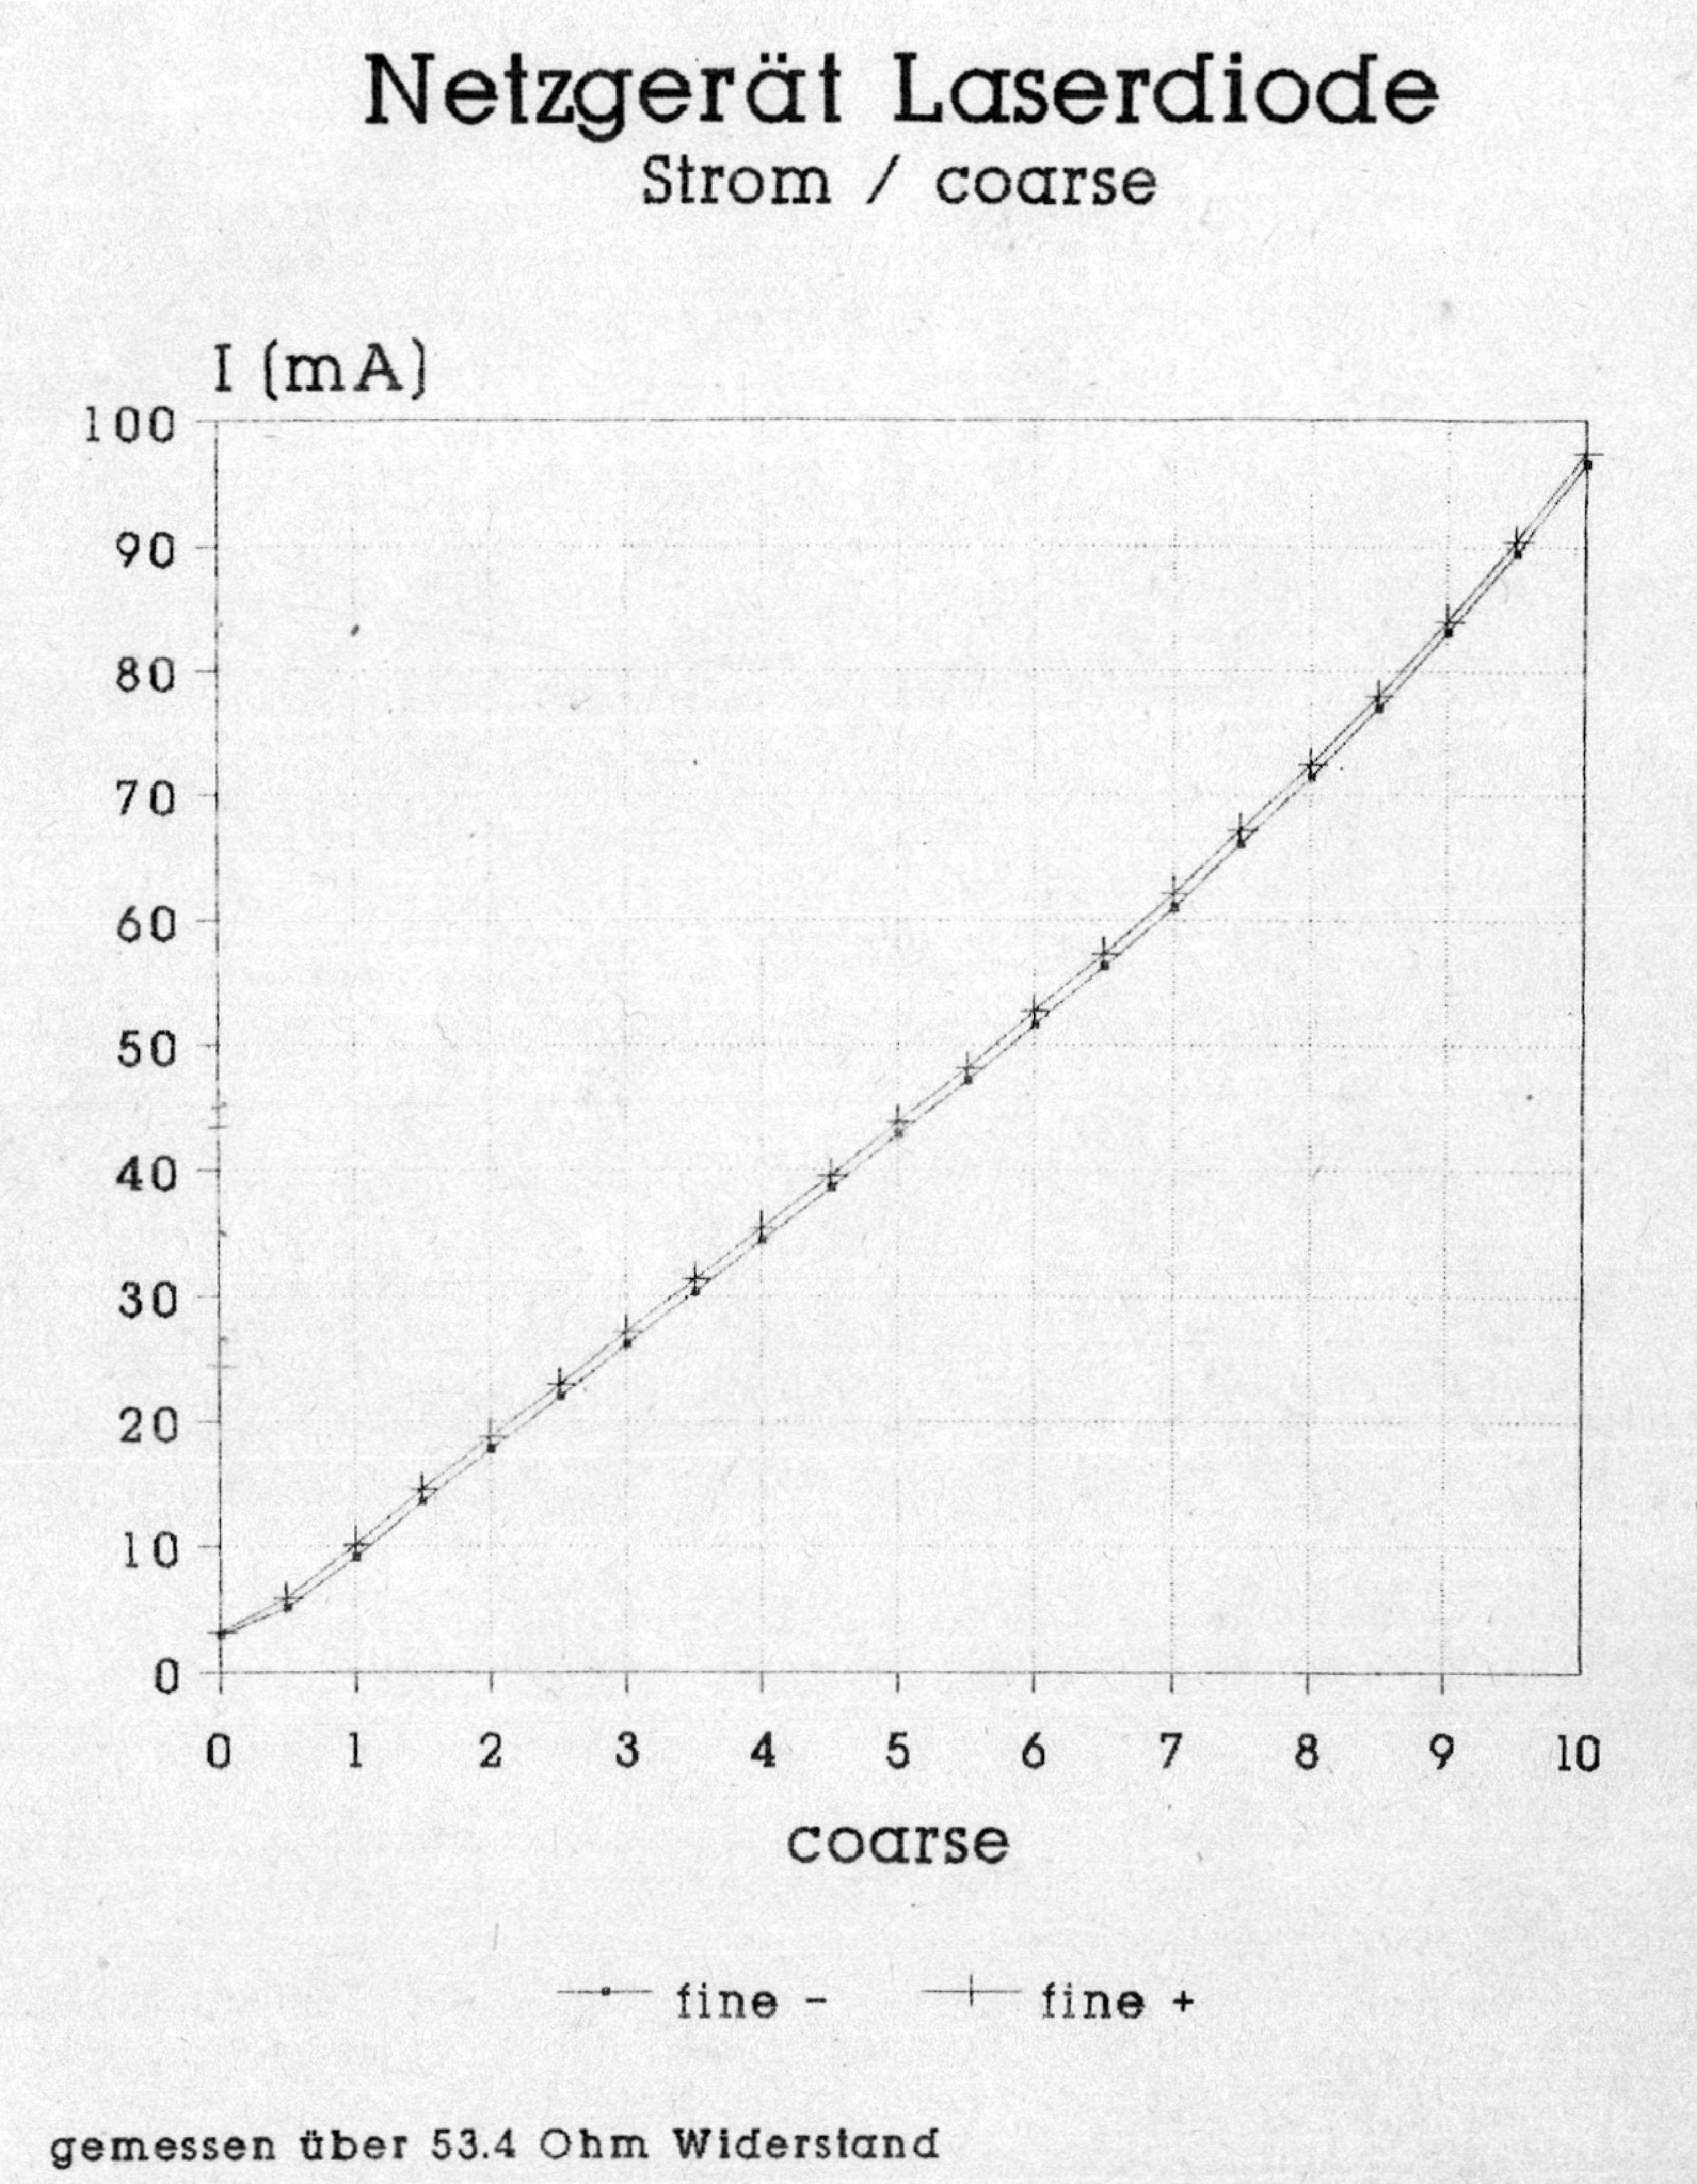
\includegraphics[width=0.85\textwidth]{figures/Stromkennlinie_Laserdiode.pdf}
        \caption{Zusammenhang zwischen dem \textit{Coarse} und der Stromstärke des Netzteils des Diodenlasers.}
        \label{fig:netzteil-kennlinie}
      \end{figure}
  \end{appendices}

\end{document}
